\subsection{Unendliche Reihen} 
\subsubsection{Grundbegriffe}\label{2.1.3}
\paragraph{Def. 6:} 
Gegeben sei die Zahlenfolge $(a_n)_n \geq n_0, \; n\in \mathbb{N}$. Die Zahlenfolge $(S_n)_n \geq n_0$ mit $S_{n_0}:=a_{n_0}, \; S_{n_0 + 1} := a_{n_0}+a_{n_0 +1}, \; S_{n_0 +2} := a_{n_0} + a_{n_0 +1} + a_{n_0 +2}, \; ..., \; S_n=a_{n_0}+a_{n_0 +1} +...+a_n$ (\emph{Partialsumeenfolge}) heißt \emph{unendliche Reihe}.\\
Bezeichnung: $\boxed{\sum_{n=n_0}^{\infty} a_n}$
\begin{itemize}
\item Die Zahlen $a_n$ heißen Glieder der Reihe, die Zahlen $S_n$ heißen Partialsummen der Reihe
\item Ist die Reihe konvergent, d.h. die Folge $(S_n)$ ist konvergent, so heißt $s:=\lim_{n\to \infty}S_n=: \sum_{n=n_0}^{\infty} a_n$ die Summe der Reihe
\item Die Reihe heißt (bestimmt oder unbestimmt) divergent, wenn die Partialsummen die entsprechende Eigenschaft haben.
\end{itemize}
Bemerkung: Oft $n_0=0$ oder $=1$
\subparagraph{Bsp. 6:} $a_n=a q^n$ mit $a\not = 0, q \not = 0, n=0,1,2,...$\\
$(a_n)=(a, aq, aq^2, aq^3,...)$ (\emph{geometrische Zahlenfolge})\\
$(S_n)=\sum_{n=0}^\infty aq^n$ (\emph{geometrische Reihe})\\
$= (\underbrace{a}_{s_0}, \underbrace{a+aq}_{s_1}, \underbrace{a+ aq+ aq^2}_{s_2}, ...)$\\
$S_n=a + aq + aq^2 + aq^3+...+aq^n \quad | \cdot q$\\
$S_nq=aq+aq^2+aq^3+aq^4+...+aq^{n+1}$\\
Beide Zeilen voneinander abgezogen:\\
$S_n-S_nq = a - aq^{n+1}\\
S_n(1-q) = a - aq^{n+1} \quad | : (1-q) \text{ falls }q\not = 1\\
\boxed{S_n = a\cdot \frac{1-q^{n+1}}{1-q}}$ (\emph{Summenformel für die endliche geometrische Reihe} mit Anfangsglied $a$ und $n+1$ Summanden)\\
$\Rightarrow \lim_{n\to \infty}S_n=\frac{a}{a-q}$ falls $|q|<1$
$\Rightarrow$ Summe der unendlichen geometrischen Reihe:\\
$\boxed{\sum_{n=0}^\infty a q^n=\frac{a}{1-q}}$ für $|q|<1$.\\
z.B. $0,\overline{72}=0,727272...=\frac{72}{100}+\frac{72}{10.000}+\frac{72}{1.000.000}+...=\frac{72}{99}=\frac{8}{11}$

\subparagraph{Bsp. 7:} $\sum_{n=1}^\infty \frac{1}{n}=1+\frac{1}{2}+\frac{1}{3}+...$ heißt \emph{harmonische Reihe}. Offensichtlich ist $(S_n)$ streng monoton wachsend. Man kann zeigen, dass $(S_n)$ nicht beschränkt ist. Aus Satz 3 folgt: die harmonische Reihe ist bestimmt divergent.\\
Schreibweise: $\sum_{n=1}^\infty \frac{1}{n}=\infty$

\paragraph{Def. 7:} Die Reihe $\sum_{n=n_0}^\infty a_n$ heißt
\begin{enumerate}[label=(\alph*)]
\item absolut konvergent, falls $\sum_{n=n_0}^\infty|a_n|$ konvergent ist.
\item bedingt konvergent, falls $\sum_{n=n_0}^\infty a_n$ konvergent, aber $\sum_{n=n_0}^\infty |a|$ nicht konvergent ist.
\end{enumerate}

\paragraph{Satz 5:} $\sum_{n=n_0}^\infty a_n$ absolut konvergent $\Rightarrow$ $\sum_{n=n_0}^\infty a_n$ konvergent.
\subparagraph{Diskussion:}
\begin{enumerate}
\item Die Umkehrung gilt im Allgemeinen nicht. Es gibt konvergente Reihen, die nicht absolut konvergieren. Z.B. $\sum_{n=1}^\infty (-1)^{n-1}\frac{1}{n}=1-\frac{1}{2}+\frac{1}{3}-\frac{1}{4}+...$
\item Für Reihen mit nicht-negativen Gliedern ($a_n \geq 0$ für alle $n$) ist absolute Konvergenz identisch mit (gewöhnlicher) Konvergenz. Für solche Reihen gilt entweder $\sum_{n=n_0}^\infty a_n<\infty$ [(absolut) konvergent] oder $\sum_{n=n_0}^\infty a_n = \infty$ [bestimmt divergent].
\end{enumerate}

\subsubsection{Konvergenzkriterien}
\begin{enumerate} [label= \arabic*., wide]
\item Notwendiges Konvergenzkriterium
\paragraph{Satz 6:} $\sum_{n=n_0}^\infty a_n$ konv. $\Rightarrow$ $\lim_{n\to \infty} a_n = 0$\\
bzw.: $(a_n)$ konvergiert $\Rightarrow$ $\sum_{n=0}^\infty a_n$ divergiert 
\subparagraph{Beweis:} $a_n = S_n - S_{n-1}$\\
$\Rightarrow \lim_{n\to \infty}a_n = \lim_{n\to\infty}S_n - \lim_{n\to\infty}S_{n-1}=s-s=0$
\subparagraph{Bemerkung:} 
\begin{enumerate}
\item Bedingung $\lim_{n\to\infty}a_n = 0$ ist notwendig, aber nicht hinreichend. Z.B. $a_n=\frac{1}{n}$, dann $\lim_{n\to\infty}a_n=0$ aber $\sum_{n=1}^\infty a_n=\infty$
\item Anwendung des Satzes meist in logisch äquivalenter Form: $\lim_{n \to \infty} a_n \not = 0 \Rightarrow \sum_{n=n_0}^\infty a_n$ divergiert
\end{enumerate}

\subparagraph{Bsp. 8:} $\sum_{n=1}^\infty \left(\frac{n}{10n-1}\right)^{50}$\\
$a_1=1,94\cdot 10^{-48}, a_2=1,3 \cdot 10^{-49}, ...$\\
$\lim_{n\to\infty}a_n=\lim_{n\to\infty}\left(\frac{n}{10-\frac{1}{n}}\right)^{50}\not = 0$\\
$\Rightarrow$ Reihe divergent (sogar besimmt divergent, da alle $a_n \geq 0$)

\item Hinreichendes Kriterien
\begin{enumerate}[label=(\Alph*),wide]
\item \emph{Leibnitzkriterium für alternierende Reihen}
\paragraph{Satz 7:} Sei $(b_n)$ Folge mit 
\begin{itemize}
\item $b_n \geq b_{n+1} > 0$ für alle $n \in \mathbb{N}$
\item $\lim_{n\to\infty} b_n = 0$
\end{itemize}
Dann ist $\sum_{n=0}^\infty(-1)^n b_n=b_0-b_1+b_2-b_3+...$ konvergent. D.h. wenn die Beträge $b_n$ der Glieder einer alternierenden Reihe mit $a_n = (-1)^n b_n$ eine Nullfolge bilden, dann ist die Reihe konvergent.\\
Weiter gilt: $|s-S_n| \leq | a_{n+1} |$\\
Also ist der Fehler bei der Approximation von $s$ durch $S_n$ beschränkt durch den Beträg von $a_{n+1}$.

\subparagraph{Bsp. 9:} $\sum_{n=1}^\infty (-1)^{n-1} \frac{1}{n}=1-\frac{1}{2}+\frac{1}{3}-\frac{1}{4}+...$ (alternierende harmonische Reihe)\\
$s_1=1, \; s_2=0,5, \; s_3\approx 0,83, \; s_4\approx 0,583, \; s_5\approx 0,78, \; s_6\approx 0,62$\\
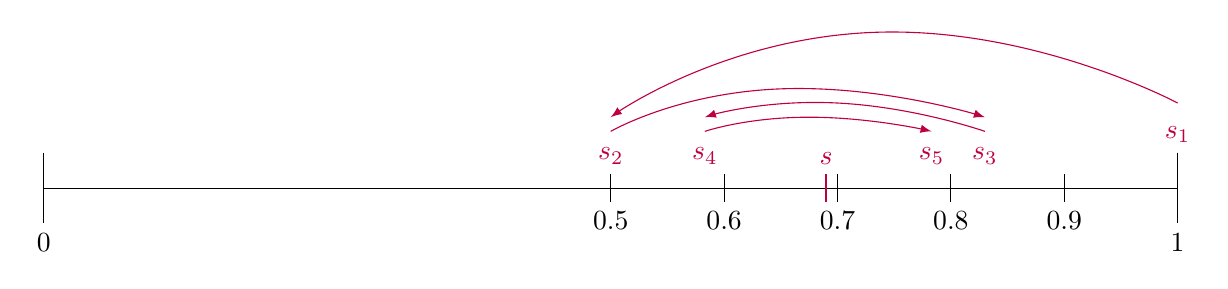
\begin{tikzpicture}[scale=.9]
\draw (0,0) -- (16,0);
\foreach \x in {0,1}{
	\draw (\x*16, 0.5) -- (\x*16,-0.5) node[below]{$\x$};
}
\foreach \x in {0.5,0.6,0.7,0.8,0.9}{
	\draw (\x*16, 0.2) -- (\x*16,-0.2) node[below]{$\x$};
}

\node[above, purple] at (16,0.5) {$s_1$};
\node[above, purple] at (0.5*16,0.2) {$s_2$};
\node[above, purple] at (0.83*16,0.2) {$s_3$};
\node[above, purple] at (0.583*16,0.2) {$s_4$};
\node[above, purple] at (0.783*16,0.2) {$s_5$};

\node[above, purple] at (0.69*16,0.2) {$s$};
\draw[purple, thick] (0.69*16, 0.2) -- (0.69*16,-0.2);

\draw [-latex, purple] plot[smooth, tension=1] coordinates {(16,1.2) (11.8,2.2) (8,1)};
\draw [-latex, purple] plot[smooth, tension=1] coordinates {(8,0.8) (10.4,1.4) (0.83*16,1)};
\draw [-latex, purple] plot[smooth, tension=1] coordinates {(0.83*16,0.8) (11.2,1.2) (0.583*16,1)};
\draw [-latex, purple] plot[smooth, tension=1] coordinates {(0.583*16,0.8) (10.8,1) (0.783*16,0.8)};
\end{tikzpicture}\\
Man kann zeigen: $s=\ln 2 = 0,6931$
\item \emph{Verleichskriterien für Reihen mit nicht-negativen Gliedern}
\paragraph{Satz 8:} (Majoranten-Kriterium)\\
Seien $(a_n)_{n\geq n_0}, (b_n)_{n\geq n_0}$ Folgen mit $0 \leq a_n \leq b_n$ für alle $n\geq n_1 \geq n_0$ und $\sum_{n=n_0}^\infty b_n < \infty$ (d.h. konvergent). \\
Dann $\sum_{n=n_0}^\infty a_n < \infty$ (d.h. konvergent).

Die Reihe $\sum _{n=n_0}^\infty b_n$ heißt dann konvergente Majorante zur Reihe $\sum_{n=n_0}^\infty a_n$.\\
Beweisidee: $0\leq a_n \leq b_n \rightsquigarrow 0 \leq \sum _{n=n_0}^\infty a_n \leq \sum _{n=n_0}^\infty b_n \leq \infty $
\paragraph{Satz 9:} (Minoranten-Kriterium)\\
Seien $(a_n)_{n\geq n_0}, (b_n)_{n\geq n_0}$ Folgen mit $0 \leq b_n \leq a_n$ für $n\geq n_1 \geq n_0$ und $\sum_{n=n_0}^\infty b_n = \infty$ (d.h. divergent)\\
Dann $\sum_{n=n_0}^\infty a_n = \infty$ (also auch divergent)\\
Die Reihe $\sum_{n=n_0}^\infty b_n$ heißt divergente Minorante der Reihe $\sum_{n=n_0}^\infty a_n$.\bigskip\\
Eine nützliche Vergleichsreihe für die Anwendung der Sätze 8 und 9 ist:\\
$\boxed{\sum_{n=1}^\infty \frac{1}{n^\lambda}= \begin{cases}
\text{konvergent} & \text{für }\lambda > 1\\
\text{divergent} & \text{für }\lambda \leq 1
\end{cases}}$
\subparagraph{Bsp. 10:} Man untersuche das Konvergenzverhalten der folgenden Reihe:
\begin{enumerate}[label=\alph*.)]
\item $\sum_{n=1}^\infty \underbrace{\frac{1}{n^2-n+1}}_{a_n}$ (Vermutung: Verhalten wie $\sum \frac{1}{n^2}$ wegen der Dominanz der höchsten Potenz)\\
Wir versuchen eine konvergente Majorante zu finden.\\
$a_n=\frac{1}{n^2-n+1}\geq \frac{1}{n^2-\frac{n^2}{2}}$ (wegen $n\geq \frac{n^2}{2}$ für $n\geq 2$)\\
Somit $\frac{1}{n^2-\frac{n^2}{2}}= \frac{2}{n^2}=:b_n$\\
Mit der Vergleichsreihe gilt: $\sum_{n=1}^\infty b_n = 2 \sum_{n=1}^\infty \frac{1}{n^2}$ ist konvergent.\\
$\overset{\text{Satz 8}}{\Longrightarrow} \sum_{n=0}^\infty a_n$ ist konvergent, sogar absolut konvergent, da $a_n\geq 0 \; (n \in \mathbb{N})$
\item $\sum_{n=1}^\infty \frac{n^2+4}{n^3+n^2+31}$ (Vermutung: divergent, da Verhalten wie $\sum \frac{n^2}{n^3}=\sum \frac{1}{n}$)\\
Wir versuchen divergente Minoranten zu finden.\\
$a_n = \frac{n^2+4}{n^3+n^2+31}\geq ... \geq \frac{1}{3n}=: b_n$ (für $n\geq 4$)\\
Wieder gilt mit der Vergleichsreihe: $\sum b_n$ divergent. Also folgt mit Satz 9: $\sum_{n=1}^\infty a_n$ divergent.
\end{enumerate}
\item \emph{Quotienten- und Wurzelkritierien}
\paragraph{Satz 10:} (Quotientenkriterium)\\
Sei $(a_n)_{n\geq n_0}$ eine Folge, so gilt:\\
$\boxed{\lim_{n\to\infty}\left|\frac{a_{n+1}}{a_n}\right|\begin{cases}
<1\\
>1
\end{cases}\Rightarrow \sum_{n=n_0}^\infty a_n \text{ ist}\begin{cases}
\text{absolut konvergent}\\
\text{divergent}
\end{cases}}$
\paragraph{Satz 11:} (Wurzelkriterium)\\
Sei $(a_n)_{n\geq n_0}$ eine Folge, so gilt:\\
$\boxed{\lim_{n\to\infty} \sqrt[n]{|a_n|} \begin{cases}
<1\\
>1
\end{cases}\Rightarrow \sum_{n=n_0}^\infty a_n \text{ ist}\begin{cases}
\text{absolut konvergent}\\
\text{divergent}
\end{cases}}$
\subparagraph{Bemerkung:} Falls in Satz 10 oder 11 $\lim ... =1$ gilt, so ist mit diesem Kriterium keine Konvergenzaussage möglich.

\subparagraph{Bsp. 11:}
\begin{enumerate}[label=\alph*.)]
\item $\sum_{n=2}^\infty \underbrace{\left( \frac{1}{\ln(n)}\right)^n \cdot (-1)^n}_{a_n}$\\
Wegen $\sqrt[n]{|a_n|}=\frac{1}{\ln n} \overset{n\to\infty}{\longrightarrow} 0 $ liefert das Wurzelkriterium, dass die Reihe absolut konvergent ist.
\item $\sum_{n=1}^\infty \frac{(-1)^n (2n)!}{(n!)^2}$\\
Wegen $\left|\frac{a_{n+1}}{a_n}\right|=\frac{\frac{(2(n+1))!}{((n+1)!)^2}}{\frac{(2n)!}{(n!)^2}}=\frac{(2n+2)!}{((n+1)!)^2}\cdot \frac{(n!)^2}{(2n)!}=\frac{(2n+2)(2n+1)(n!)^2}{(n+1)^2 (n!)^2}=\frac{(2n+2)(2n+1)}{(n+1)^2}
=\frac{4n^2+4n+2n+2}{n^2+2n+1}\overset{n\to\infty}{\longrightarrow} 4$\\
Daher ist die Reihe divergent.
\end{enumerate}
\end{enumerate}
\end{enumerate}

\subsubsection{Rechenregeln}
\begin{itemize}
\item $\sum_{n=n_0}^\infty a_n$ und $\sum_{n=n_0}^\infty$ konvergent mit Summe $a$ und $b$, dann gilt: 
\begin{itemize}
\item $\sum_{n=n_0}^\infty (a_n+b_n)= a + b$
\item $\sum_{n=n_0}^\infty c\cdot a_n= c\cdot a$
\end{itemize}
\item $\sum_{n=n_0}^\infty a_n$ absolut konvergent $\Leftrightarrow$ die Glieder $a_n$ lassen sich beliebig umordnen, ohne dass sich die Summe ändert.
\item $\sum_{n=n_0}^\infty a_n$ und $\sum_{n=n_0}^\infty b_n$ absolut konvergen mit Summen $a$ und $b$, dann gilt:
\begin{itemize}
\item $\left(\sum_{i=0}^\infty a_i\right)\cdot \left( \sum_{j=0}^\infty b_j\right)=\sum_{i=0}^\infty  \sum_{j=0}^\infty a_i b_j=a\cdot b \qquad \left( =\sum_{n=0}^\infty  \sum_{i=0}^\infty a_i b_{n-i} \quad \text{Cauchy-Produkt}\right)$
\end{itemize}
\end{itemize}